\section{Regression testing, Package management and Release management}\label{gap-infra}

As well as developments in the core system and in packages, we have
dedicated considerable effort to improving our infrastructure and processes. 
In this section we describe developments in the technical processes
which support our developers (especially package developers),
connect them to our user community, and aim to 
ensure the robustness and quality of the integrated system.
\comment{Social aspects including community building, user training
and technical support will be described in D2.15 (check that)}

\TODO{Think about the structure of this section -- at the moment it's
  not clear where it is going or what point is being made. Are we
  describing the overall situation, or developments made during \ODK
  AK: shortened and reordered; will need another pass}

\subsection{Regression testing}\label{testing}

\emph{Regression testing} is a software engineering technique which
checks (preferably in an automated way)
that new changes do not break functionality that 
worked previously. If a change breaks a test, that is 
a \emph{regression}. In \GAP, regressions may occur
when a change causes an incorrect result, or a crash, or an unwanted error
message; in addition, there may be \emph{performance regressions}
and \emph{memory regressions} where a test becomes slower, or uses
much more memory after a change.

Regression testing has been embedded into all the \GAP developments
from the very beginning of the project, being based on the existing
practices used by the \GAP project in one or another form since 1980s,
and automated in the first half of the current decade by 
using the \href{https://jenkins.io/}{\sf Jenkins} system installation
at USTAN to regularly run \GAP testsuite for the \GAP development 
version and release candidates.
{\sf Jenkins} can keep and archive of test logs, and notify
developers when tests fail; however, the biggest limitation of our setup are that
it is not public and can be accessed only within St Andrews. 
\GAP developers came to an understanding 
that one of the limiting factors (not only for the testing, but for
the \GAP development in general) was that while \GAP is an open source 
software, it does not follow an open development model and does not
have a public source code repository, and just before the start of
the project established a public source code repository for \GAP
on GitHub at \url{https://github.com/gap-system/gap}. 

In the duration of the OpenDreamKit project we, together with other
contributors to the \GAP project, consolidated \GAP development 
around GitHub and its tool ecosystem.
Hosting GAP repository on GitHub and eventual establishing of a number
of other repositories under the gap-system and gap-packages 
organizations (\url{https://github.com/gap-system} and 
\url{https://github.com/gap-packages}), and encouraging package authors 
to follow the same practices (see \url{https://gap-packages.github.io/})
to find some further packages that are having public source code 
repositories elsewhere) allowed us to bring our regression testing
up to the next level.

\TODO{maybe mention that we can break out onto GitLab if GitHub
changes in some unacceptable way} 

We made use of \href{https://travis-ci.org/}{Travis CI} and
\href{https://www.appveyor.com/}{AppVeyor} which are 
free (for open source projects) continuous integration platforms 
that can be used to build and test software projects hosted at GitHub.
\emph{Continuous Integration}, usually abbreviated as {\bf CI} is the process
automated building and testing for every performed or suggested changes to 
the source code repository. Using Travis and AppVeyor, one can test changes proposed
in a pull request \emph{before} they are merged into the main repository.
At the moment, we use Travis CI for tests on Linux and OS X, and 
AppVeyor for tests on Windows.

In addition to that, we started to use \href{https://codecov.io/}{Codecov}
platform to collect \emph{code coverage} reports for GAP to ensure that our
regression tests exercise GAP codebase at an acceptable level, and then
the changes which are submitted via pull request are actually being tested
by Travis CI. Making these results easily obtainable and publicly available
had a great effect on the community. Adding new tests to improve code coverage
is a useful task for new contributors to familiarize themselves with the
project setup. Making coverage reports available for each pull requests
facilitates checking code coverage during code review and
encourages their authors to ensure that their contributions have a good
quality and their suggested changes are actually being tested. 

\TODO{Perhaps move the table with the number of lines in tests here?}
The \GAP test
suite for the core system consists of a total of 707 test files at the time of writing
totaling over $60\,000$ lines,
as well as of the tests that check the correctness of over
over $14,000$ lines of 1810 manual examples.
%% \comment{1336 mansections containing examples;
%% 1641 (ref) + 169 (tut) = 1810 examples;
%% 13262 (ref) + 940 (tut) = 14202 lines}. 
%% in doc/ref
%Read("makedocreldata.g");
%exsref := ExtractExamples(GAPInfo.ManualDataRef.pathtodoc,
%       GAPInfo.ManualDataRef.main, GAPInfo.ManualDataRef.files, "Chapter");;
%exsref := Filtered( exsref, ch -> Length( ch ) > 0 );;
%Sum(List(exsref,Length));
%Sum(List(exsref, ch -> Sum(List( ch, ex -> Length(Filtered(SplitString(ex[1],"\n"), x -> x<>""))))));
%
%% in doc/tut
%Read("makedocreldata.g");
%exsref := ExtractExamples(GAPInfo.ManualDataTut.pathtodoc,
%       GAPInfo.ManualDataTut.main, GAPInfo.ManualDataTut.files, "Chapter");;
%exsref := Filtered( exsref, ch -> Length( ch ) > 0 );;
%Sum(List(exsref,Length));
%Sum(List(exsref, ch -> Sum(List( ch, ex -> Length(Filtered(SplitString(ex[1],"\n"), x -> x<>""))))));
%%
%% 
% and some further code in the {\tt benchmarks} directory. 

\GAP package authors are recommended to 
use a similar approach to testing and to provide their own regression
tests. Many do, adding, in total over a quarter of a million lines of
further tests.

A crucial role in these developments was played by the enhanced
profiling facilities discussed 
in Subsection~\ref{gap-4.8}. 
GAP~4.8 also introduced the {\tt TestDirectory} function to find
(recursively) all {\tt .tst} files from a given directory or a list of 
directories and run them using {\tt Test}. Having ability to test
changes more efficiently also allowed us to further improve all 
tools involved in testing, making their output more informative,
and allowing test integration into various automated workflows
by a better detection of the test outcomes. % the logic seems backwards here. Better test tools let us test better, not v.v.
% What I had in mind was that once we set up the system with the
% state of the testing framework as it was, we were able to "test the testing"
% itself, and improve it - for example, by adding progress indicators,
% report time spent on GC and memory used, etc.

\TODO{We need to get to this point much sooner. AK: reduced the 
above test by half a page so far. Can we reorder -- start with the
fact that instead of cumbersome manually maintained lists and whatever
the release manager now has modern dashbaords summarising lots of
stuff. Then explain how we got there and what all the components are?}

Figure~\ref{fig:gap-core-tests} displays a part of the dashboard
available at \url{https://github.com/gap-system/gap-distribution/}.
The ``status'' buttons lead to the test reports on Travis CI, and
the ``code coverage'' buttons lead to the code coverage reports on
Codecov. The coverage is shown for the latest revision in the
corresponding branch (release branches {\tt stable-4.9} and {\tt stable-4.10},
and the master branch which is the prototype of the coming GAP~4.11 release).

\begin{figure}[!ht]
    \centering
    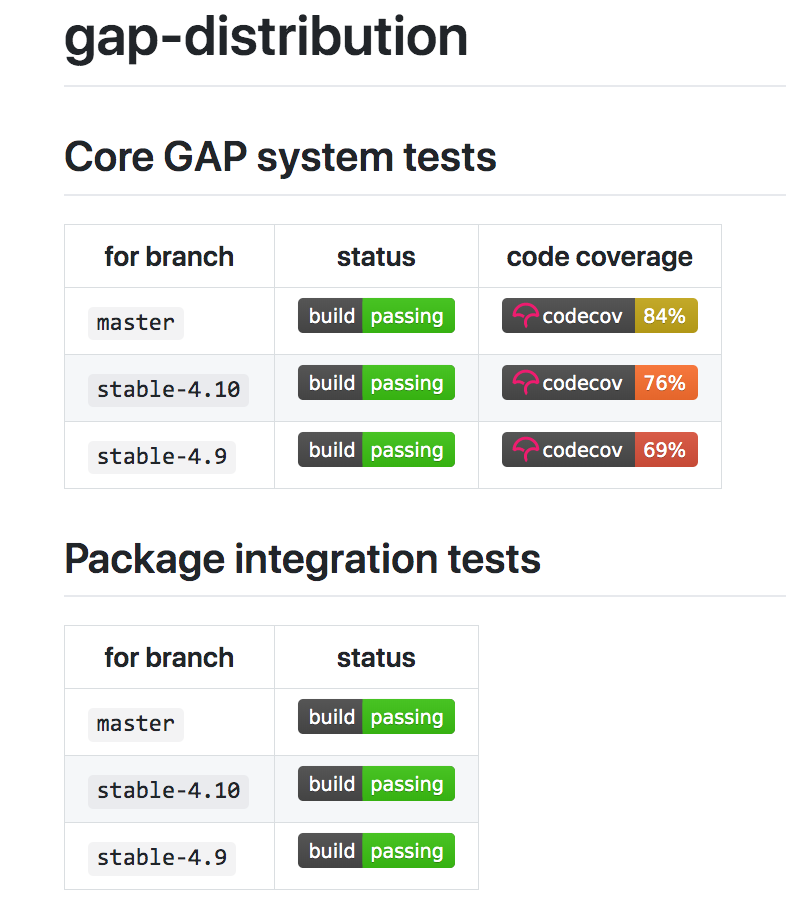
\includegraphics[width=5cm]{images/gap-core-tests}
    \caption{Dashboard with core GAP system and package integration tests}
    \label{fig:gap-core-tests}
\end{figure}

The top part of Figure~\ref{fig:gap-core-tests} shows core system GAP tests,
which are run for every change made to the repository. The bottom part shows
tests which are run once in 24 hours using a Docker container which is built
using a snapshot of the GAP development version on the moment of its creation
and a selection of \GAP packages (including their updates, not yet redistributed
with \GAP). Clicking on the ``status'' button will lead to the overview displayed
on Figure~\ref{fig:gap-docker-master-testsuite}, from where one could inspect
test logs for each of the configurations and see the diagnostics in case of a
test failure.

\begin{figure}[!ht]
    \centering
    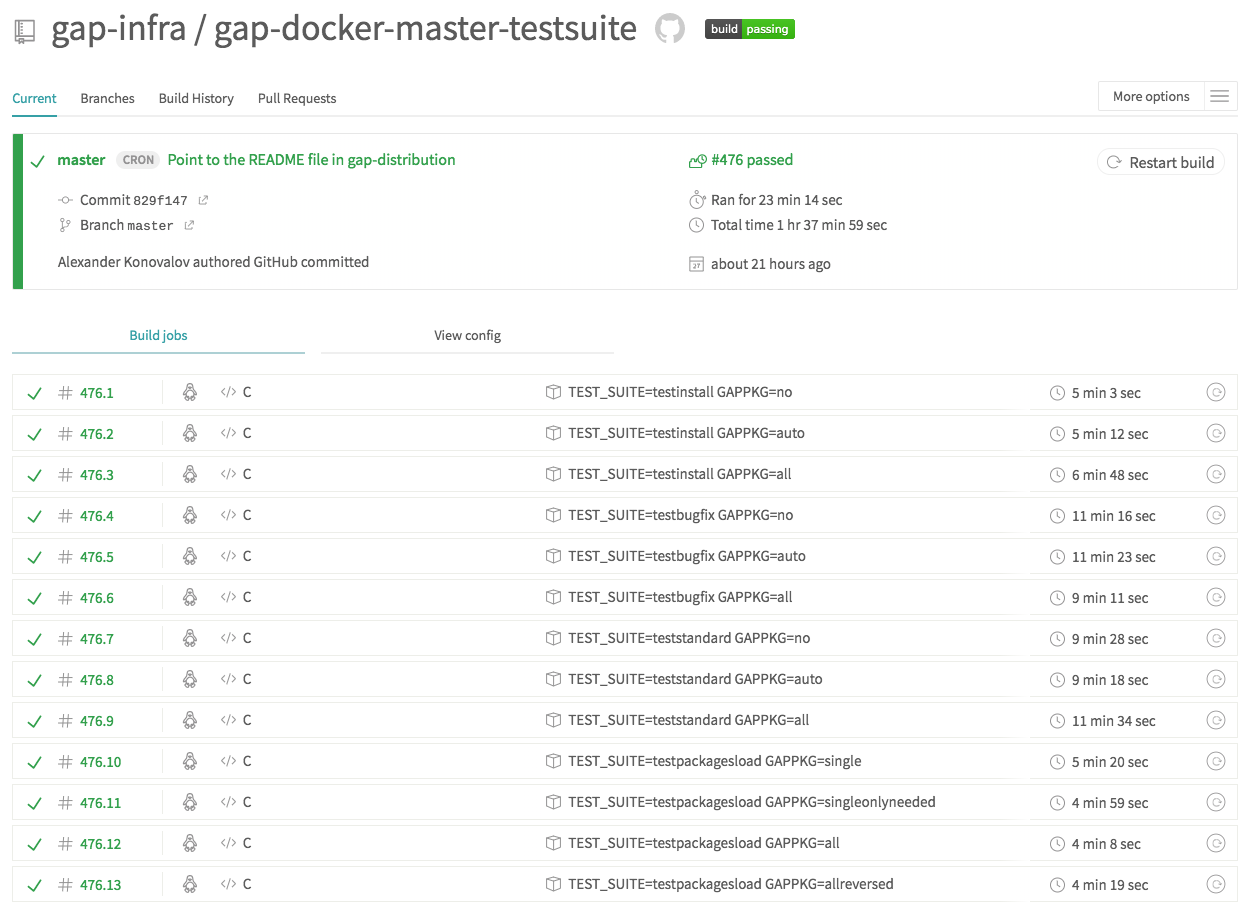
\includegraphics[width=\textwidth]{images/gap-docker-master-testsuite}
    \caption{GAP package integration tests on Travis CI}
    \label{fig:gap-docker-master-testsuite}
\end{figure}

The Docker container for the test displayed on Figure~\ref{fig:gap-docker-master-testsuite}
is one of a set of containers that we maintain for various purposes, from offering 
them as alternative distributions (see Subsection~\ref{distro}) or components for sharable
reproducible experiments (see Appendix~\ref{repro-gap}), to ways to speed up regression tests running
container-based tests on Travis CI. These containers are publicly available on Docker Hub
(see Figure~\ref{fig:gap-docker}).
\comment{The Docker stuff might deserve to be its own section}
\TODO{Refer to deliverable where Docker was previously reported}

\begin{figure}[!ht]
    \centering
    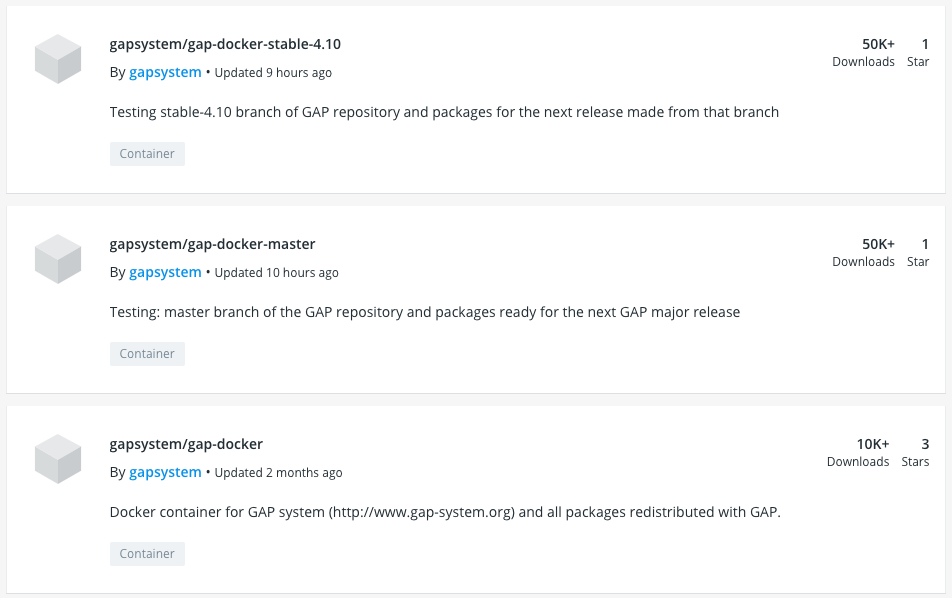
\includegraphics[width=12cm]{images/gap-docker}
    \caption{Selected \GAP Docker containers on Docker Hub}
    \label{fig:gap-docker}
\end{figure}

At the same time, we continue to use Jenkins installation in St Andrews 
for daily and weekly tests, running package updates system, wrapping and
testing release candidates and other tasks. It is also very valuable since 
it does not impose time limits on output inactivity and the overall duration
of the job; second, it allows us to log in into the test workspace for
debugging; third, with the specific \GAP setup for Windows we build it on a
machine with a Cygwin installation, and then install it on a clean Windows
machine to test there. 
